\chapter{\label{chap:impl}Implementação}

Para a implementação do simulador, foi escolhida a linguagem C++, por sua grande
flexibilidade e performance, bem como suas poderosas primitivas de controle de
cópia e modificação de objetos.

Os resultados da simulação geram um \textit{log} completo, que é analisado por
uma ferramenta separada, escrita em Python. Esta escolha foi feita pela grande
gama de bibliotecas científicas e estatísticas disponíveis para Python, que
facilitaram enormemente a geração de gráficos para este trabalho.

\section{Cenários}

\lipsum[1]

\section{Simulador}

\lipsum[1]

\subsection{Geração de Chegadas}

\lipsum[1]

\subsection{Notificação de Eventos}

\lipsum[1]

\subsection{Atualização do Estado do Sistema}

\lipsum[1]

\section{Estatísticas}

\lipsum[1]

\section{Geração de Relatórios}

\lipsum[1]

\subsection{Geração de Gráficos}

Os gráficos são gerados com auxílio da biblioteca Seaborn~\cite{seaborn},
implementada na linguagem Python. Esta biblioteca possui primitivas poderosas de
cálculos estatísticos e geração de gráficos, garantido a corretude da análise
dos resultados com um esforço reduzido.

Pode-se ver no algoritmo~\ref{alg:seaborn} um exemplo da expressividade desta
ferramenta.

\begin{algorithm}[htb]
  \centering
    \begin{minted}[frame=lines,framesep=2mm,linenos,fontsize=\small]{python}
    def averageTravelTime(data):
        data['travelTime'] = data['dropoffTime'] - data['pickupTime']
        g = sns.FacetGrid(data, col='dropoffFloor', row='arrivalFloor')
        g = g.map(sns.barplot, "travelTime", orient='v')
    \end{minted}
  \caption{Geração de gráfico de matriz de tempo de espera.}
  \label{alg:seaborn}
\end{algorithm}

Na linha 2 do algoritmo~\ref{alg:seaborn}, utiliza-se a ferramenta de
vetorização para calcular-se a diferença entre o tempo de entrega do passageiro
(\textsf{dropoffTime}) e o tempo em que ele foi pego pelo elevador
(\textsf{pickupTime}). Note que nem mesmo um \textit{loop} é necessário. A
biblioteca infere isto e calcula para todos os valores.

Nas linhas seguintes, apenas diz-se o que se quer nas colunas e linhas do
gráfico, e o que deve ser representado pelas barras verticais.

Um exemplo de gráfico gerado por este código está na Figura~\ref{fig:seaborn:exemplo}.

\begin{figure}[htb]
  \centering
  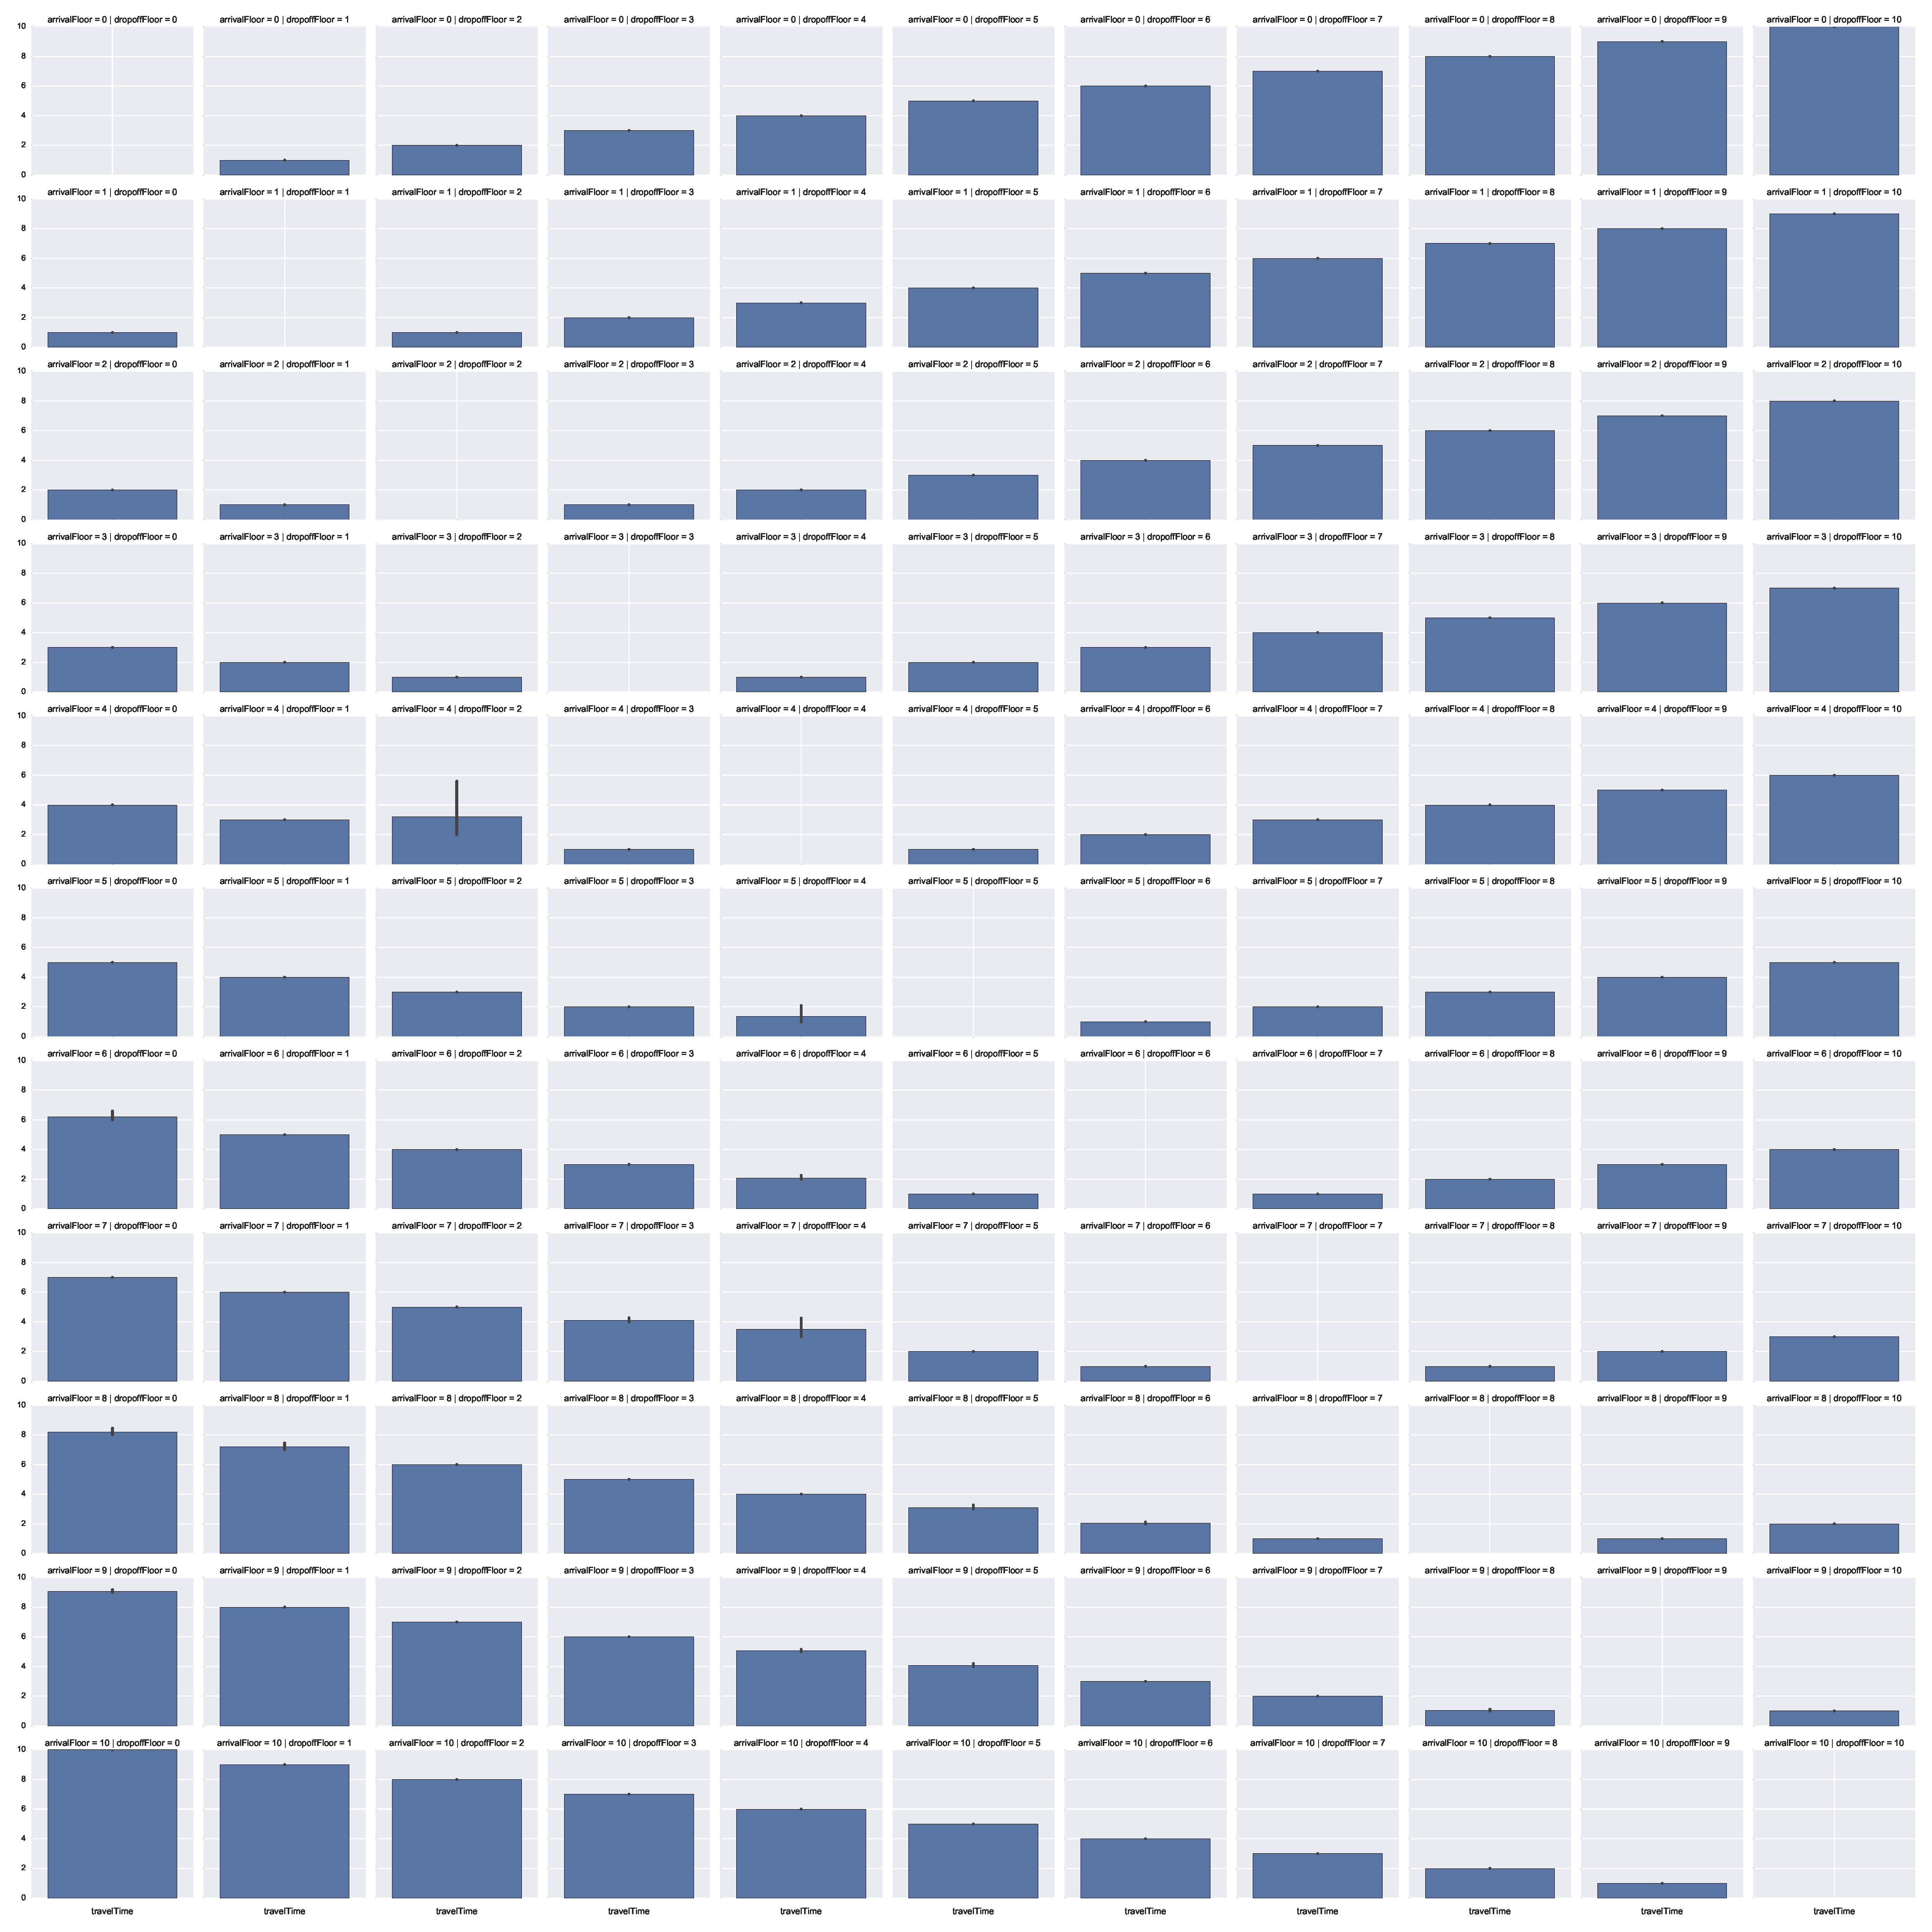
\includegraphics[scale=0.1]{img/seaborn_example.eps}
  \caption{Um exemplo de gráfico gerado pelo código do
    Algoritmo~\ref{alg:seaborn}.}
  \label{fig:seaborn:exemplo}
\end{figure}

\section{Schedulers}

\lipsum[1]

\subsection{Classe Base}

\lipsum[1]

\subsection{Simple}

\lipsum[1]

\subsection{Planning}

\lipsum[1]

\section{Funções de Custo}

\lipsum[1]

\subsection{Classe Base}

\lipsum[1]

\subsection{Dummy}

\lipsum[1]

\subsection{Random}

\lipsum[1]

\subsection{Nearest Neighbour}

\lipsum[1]

\subsection{Nearest Neighbour Melhorado}

\lipsum[1]

\subsection{Weighted}

\lipsum[1]